\section{CAnalytics}
\begin{figure*}
	\centering
	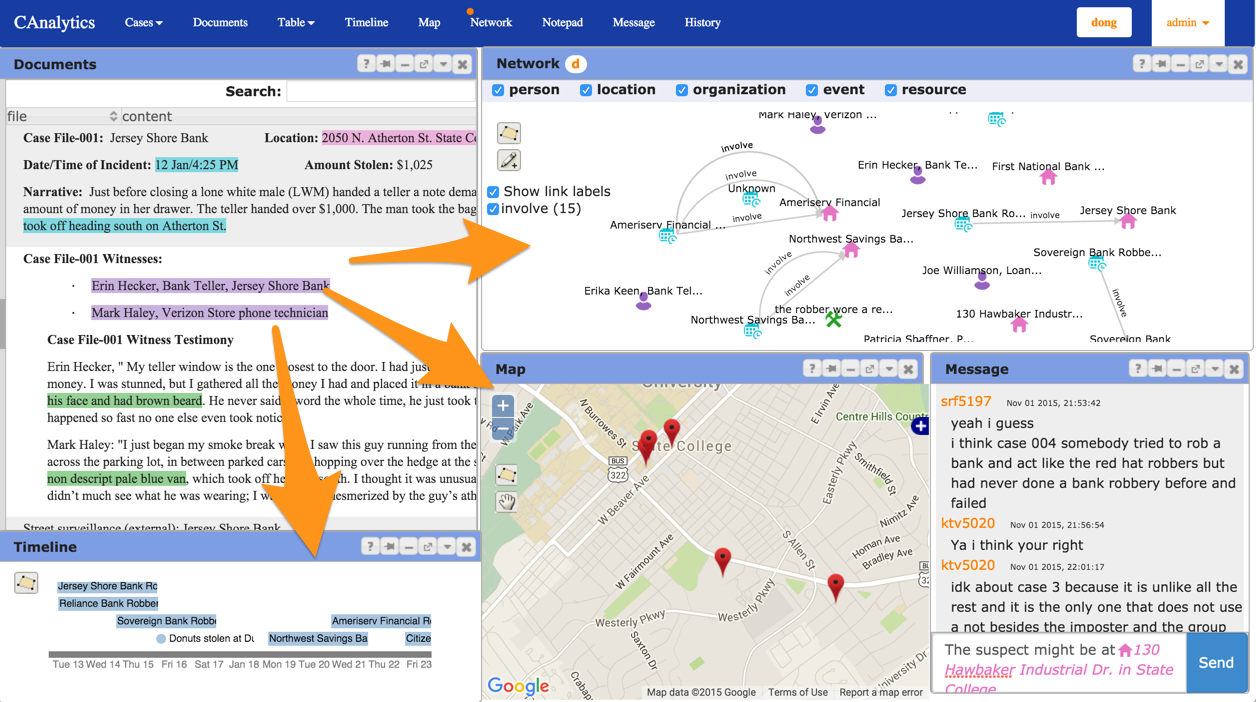
\includegraphics[height=3in]{img/ca_annotation}
	\caption{CAnalytics user interface}
	\label{fig:canalytics}
\end{figure*}

We developed a collaborative information analysis tool, CAnalytics, to support distributed teams of analysts in identifying, visualizing, integrating and assessing facts from multiple sources. The design is informed by existing entity-based information systems \cite{Bier2010} and real-time collaborative systems \cite{Goyal2014}, as well as by findings of prior paper prototype studies of teams performing information analysis tasks \cite{Carroll2013}, Chin et al's \cite{Chin2009} study of intelligence analysts, and Kang and Stasko's \cite{Kang2011} field study of analysts-in-training. The following are explicit design choices we made to enhance collaborative evidence collection, collaborative evidence schematization, and overall coordination and communication respectively. 


\subsection{Semantic annotation for evidence collection}
CAnalytics supports evidence collection through annotation. In the document view users can highlight and annotate information about people, location, events, etc., as well as relationships between them. Unlike in other entity-based systems e.g. \cite{Bier2010}, we use manual annotation for objects of interest. This allows for greater user control in information gathering. Users can decide their own information granularity and information interest that best suits their ad-hoc analytic needs. 

We call it ``semantic'' annotation because the annotation is not only a highlight mark on document text (as usually is), but users can add attributes to annotations, e.g. add time attribute in event, coordinate in location. Thus each annotation is a data object that embeds information of evidence entity. Users can also make reference to other objects in the attribute; for example, users can add people objects involved in an event. A few utilities are available to facilitate data input, e.g. geocoding address, auto-completion of existing data objects. Annotation also records the source where a data object was created---users can always re-access the data objects in its original context of the problem document, a critical requirement emphasized by \cite{Chin2009}.

Our tool supports real-time collaborative editing, similar to the Google Tools. Users can open several concurrent editors to collaboratively edit multiple annotations and events. User created data objects are immediately shared within a team. As far as we know, this tool is the first to support multi-concurrent editing, which we think can improve fine grain coordination and awareness in complex collaborative work. The tool also includes a notepad, in which users can collaboratively compile a document, similar to Google Doc. 

In sum, users accomplish three things when creating an annotation: 1. highlight critical information in the document; 2. model data objects in preparation for later visualization and analysis; 3. connecting data object with source of document for evidence provenance. Annotations are synchronized in real time for collaborative evidence collection. 
	
\subsection{Multiple coordinated views for evidence schematization}

CAnalytics supports information analysis by automatically organizing user created objects in multiple coordinated views, including table, timeline, map, and node-link graph---tools that are most frequently used in information analysis tasks \cite{Carroll2013}. Each visualization provides a way to schematize data: timeline organizes data by time, map by location, node-link graph by relationships, and table by attributes. Figure \ref{fig:canalytics} shows an example of the multiple visualizations in our tool: when an annotation is created in the document module, with information about time, location, participants, and their relationships, a new event is created in the timeline module, a new location is created in the map module, and new people are created in the node-link graph module with a typed edges representing relationships among the people (or new edges are added to existing nodes). 

Different views are coordinated; that is, when users do a filter on a piece of information in one views, related information in other views will be highlighted. Filtering on different views/schematization provides different analytic strategies; e.g. timeline offers filtering by time, map offers filtering by location, and node-link graph offers filtering by related data objects.

Based on default view of evidence, users can continue to schematize it. For example, users can drag the nodes in the node-link graph to make clusters. Users can also create a relationship in the graph by drawing a link between two nodes and input relationship attributes. 

\subsection{Awareness features for coordination}
	
CAnalytics has a number of awareness features, including real time data sharing, a notification system,  a design we named ``tool coordinator'', a message tool, and a history tool. As mentioned before, annotations and data objects created by collaborators are immediately shared. Annotations will be highlighted in the exact position on teammate's document view, indicating which part of the document teammates are working on. Data objects will be visualized in multiple views together with existing data, keeping latest gathered information available to the team. A notification system sends individual's actions to the team, in the form of a text box in the top right corner of the workspace, keeping the team up to date with collaborator's actions. To reduce notification noise, instead of broadcasting whatever actions, we define a set of rules to determine which actions will be notified. For example, the action that creates an entity will be notified, but that re-layouts a view will not. Tool coordinator refers to a small indicator on the tool menu bar, suggesting who is working on the tool. 

The message tool enables real time team communication. Chat history is also persistent for traceability. We design a ``mention'' feature---users can refer to created entities and relationships in the workspace when they are composing a message. We believe this will improve communication efficiency because analysts are often observed to mention critical information entities in face-to-face discussion. \cite{Carroll2013}. When the message receiver hovers over the object, attributes of the object shows up, ensuring that the team is talking about the same thing (as \cite{Carroll2013} observed, one frequent collaboration breakdown is misunderstanding of the object in discussion). 

The system maintains a persistent log of time-stamped individual activities. A history tool presents who did what to which object at when. Together with the notification system, users who work synchronously can be informed of others' activity continuingly, and be aware of the bigger picture of team's activity; users who work asynchronously will be able to use the history to reconstruct their work status and become aware of changes beyond the point of their last interaction. 
		
Different from awareness features developed in existing systems which are simply read-only text, the awareness information in our system is closely integrated with the analytic environment. For example, data objects that are changed and presented in the history view are clickable links. Users can hover over to read detailed attributes and click to do a filter on the object.  
		

The system also includes a simple notepad implementation to support collaborative hypothesis generation. We integrate Etherpad \footnote{Etherpad url}, an open sourced collaborator editor much like Google Doc, for teams to compose their hypotheses. Users can insert tables (e.g. an ACH matrix) and images (views of evidence schematization). However, by the time of this study, we have not developed any advanced features specific for the task of information analysis, and usage of the editor for hypothesis generation is not the emphasis of this paper. 
